The investigation of quantum phase transitions in strongly correlated systems is an important and fascinating area of research. The one-dimensional Bose-Hubbard model is a minimal bosonic many-particle model that captures the essential physics of interacting bosons on a lattice \cite{kuehner_phases_1998}
\begin{equation*}
	H = -t \sum_{j} (a_j\D a_{j+1} + \hc) + \tfrac{1}{2}U \sum_j n_j (n_j-1) - \mu \sum_j n_j
\end{equation*}
and garnered significant attention due to the existence of both the Mott insulator (MI) and superfluid (SF) phases, as well as the successful application of DMRG \cite{PhysRevLett.69.2863}.

The MI\textsuperscript{\footnote{
    The MI phase is particularly notable for its role in ultracold atom experiments, where it facilitates the deterministic preparation of a single-site occupancy lattice—a critical step in quantum simulation and computation experiments \cite{choi_exploring_2016}.
}} phase is characterized by its lack of particle mobility due to strong interactions, resulting in a fixed integer number of particles per site and an energy gap for particle-hole excitations. This phase exhibits suppressed number fluctuations and localized particles, leading to short correlation lengths and an insulating behavior. In the MI phase, the correlation function $\Gamma(r) = \langle a_j^\dagger a_{j+r} \rangle$ decays \textit{exponentially} with distance (fig. \ref{fig:decay}.1). 

On the other hand, the SF phase features delocalized particles that can move freely across the lattice, leading to long-range phase coherence and the absence of an energy gap. This phase is marked by large number fluctuations and a diverging correlation length, indicating a coherent, macroscopic quantum state. In the SF phase, the correlation function $\Gamma(r)$ decays \textit{polynomially} with distance (fig. \ref{fig:decay}.3).


\begin{figure}[b]
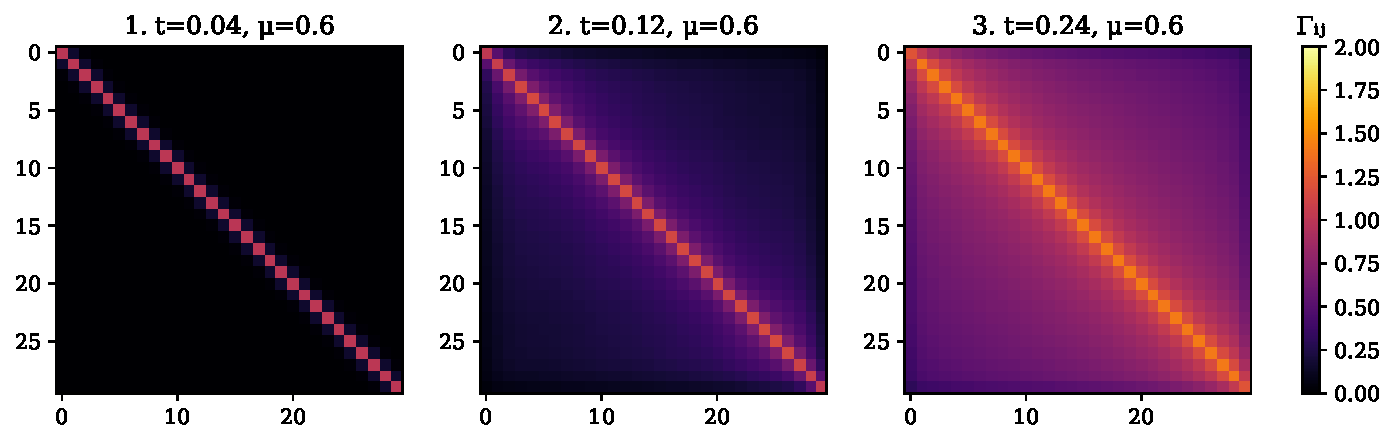
\includegraphics[width=\linewidth]{imgs/corrs.pdf}
\caption{The characteristic form of $\Gamma_{ij}$ at three points in the phase space: MI (1), critical point (2), and SF (3). The same points are used for illustration purposes throughout the text.}
\label{fig:corrmat}
\end{figure}

\section{Methodology}


In this article, we will focus on three key quantities to distinguish between these phases: the correlation length $\xi$, the average site occupancy $\langle n_j \rangle$, and the polynomial degree \( K \) with which \(\Gamma^2\) decays, following the approach in [1]. These properties provide valuable insights into the nature of the MI and SF phases. By examining these parameters, we aim to deepen our understanding of the phase transitions within the one-dimensional Bose-Hubbard model.




